\section[1977年高考数学试卷及答案(福建卷)理科]{1977年普通高等学校招生考试(福建卷)\\\Huge{理科数学}}

\begin{questions}
	\question
	\begin{enumerate}[label=(\arabic*)]
		\item 计算: \( 5 - 3 \times \left[(-3\frac38)^{-\frac13} + 1031 \times (0.25 - 2^{-2})\right] \div 9^0 \).
		      \begin{solution}
			      \begin{align*}
				      \text{原式} & = 5 - 3 \times \left[ (-3\frac38)^{-\frac13} + 1031 \times 0 \right] \div 1 \\
				                & = 5 - 3 \times (-\frac{8}{27})^{\frac13}                                    \\
				                & = 5 - \sqrt[3]{3^3 \times (-\frac{8}{27}})                                  \\
				                & = 5 + 2                                                                     \\
				                & = 7
			      \end{align*}
		      \end{solution}

		\item \( y = \dfrac{\cos{160^\circ} - \cos{170^\circ}}{\tan{155^\circ}} \)的值是正的还是负的?为什么?
		      \begin{solution}
			      \begin{center}
				      \begin{tikzpicture}
					      \begin{axis}[
							      xmin=-1, xmax=2.5*pi,
							      ymin=-2, ymax=2,
							      legend entries={$\cos{x}$, $\tan{x}$},
							      title=$\cos{x}$和$\tan{x}$的函数图像,
							      title style={anchor=north, yshift=-6cm}
						      ]
						      \addplot[domain=0:2*pi, color=blue, thick]{cos(deg(x))};
						      \addplot[domain=0:2*pi, color=red, thick]{tan(deg(x))};
					      \end{axis}
				      \end{tikzpicture}
			      \end{center}

			      \begin{enumerate}[label=\protect\circled{\arabic*}]
				      \item 余弦函数在第二象限单调递减,所以$\cos\ang{160} - \cos\ang{170} > 0$;
				      \item 正切函数在第二象限小于零,所以$\tan\ang{155} < 0$;
				      \item 综上,$y<0$.
			      \end{enumerate}
		      \end{solution}

		\item 求函数 \( y = \dfrac{\lg(2-x)}{\sqrt{x-1}} \)的定义域.
		      \begin{solution}
			      根据题意有
			      \begin{math}
				      \begin{cases}
					      2 - x > 0 \\
					      x - 1 > 0,
				      \end{cases}
			      \end{math}
			      则函数的定义域为 \( 1 < x < 2 \)
		      \end{solution}
		\item
		      \begin{minipage}[t]{0.5\textwidth}
			      如图,在梯形 \( ABCD \)中, \( DM = MP = PA, MN \parallel PQ \parallel AB \), \( DC = 2\text{cm}, AB = 3.5\text{cm} \),求 \( MN \)和 \( PQ \)的长.
		      \end{minipage}\hspace{5em}
		      \begin{tikzpicture}[baseline=(current bounding box.center)]
			      \tkzDefPoints{0/0/A, 3/0/B, 0.5/3/D, 2.5/3/C}
			      \tkzDefPointOnLine[pos={1/3}](A,D)\tkzGetPoint{P}
			      \tkzDefPointOnLine[pos={2/3}](A,D)\tkzGetPoint{M}
			      \tkzDefPointOnLine[pos={1/3}](C,B)\tkzGetPoint{N}
			      \tkzDefPointOnLine[pos={2/3}](C,B)\tkzGetPoint{Q}

			      \tkzDrawPolygon(A,B,C,D)
			      \tkzDrawSegments(P,Q M,N)

			      \tkzLabelSegment[above](D,C){$2$cm}
			      \tkzLabelSegment[below](A,B){$3.5$cm}

			      \tkzLabelPoints[left](D,M,P,A)
			      \tkzLabelPoints[right](C,N,Q,B)

		      \end{tikzpicture}

		      \begin{solution}
			      根据梯形的性质有:
			      \begin{equation*}
				      \begin{cases}
					      DC + PQ = 2MN \\
					      MN + AB = 2PQ
				      \end{cases}
			      \end{equation*}
			      计算得:
			      \begin{equation*}
				      MN = 2.5\text{cm}, PQ = 3\text{cm}.
			      \end{equation*}
		      \end{solution}
		\item 已经 \( \lg3=0.4771, \lg{x}=-3.5229 \),求 \( x \).
		      \begin{solution}
			      \begin{align*}
				       & \because \lg3                              = 0.4771                  \\
				       & \therefore \lg{\frac{3}{10}}               = \lg3 - \lg10 = -0.5229  \\
				       & \text{另有} \lg0.001                       = -3                        \\
				       & \text{则} \lg(0.001 \times \frac{3}{10} )  = -3 + (-0.5229) = -3.5229 \\
				       & \therefore x = \frac{3}{10000}
			      \end{align*}
		      \end{solution}
		\item 求 \(\displaystyle \lim_{x\to1}\frac{x-1}{x^2-3x+2} \).
		      \begin{solution}
			      \begin{align*}
				      \frac{x-1}{x^2 - 3x + 2} & = \frac{x-1}{(x-2)(x-1)} \\
				                               & = \frac{1}{x-2}
			      \end{align*}
			      则 \( \displaystyle \lim_{x\to1}\frac{x-1}{x^2-3x+2}=-1 \)
		      \end{solution}
		\item 解方程: \( \sqrt{4x+1} - 2x + 1 = 0 \).
		      \begin{solution}
			      移项得:
			      \begin{math}
				      \sqrt{4x+1} = 2x - 1
			      \end{math}

			      两边平方得:
			      \begin{math}
				      4x + 1 = 4x^2 - 4x + 1
			      \end{math}

			      整理得:
			      \begin{math}
				      4x^2 -8x = 0
			      \end{math}

			      提取同类项得:
			      \begin{math}
				      4x(x-2) = 0
			      \end{math}

			      则
			      \begin{math}
				      x_1 = 0, x_2 = 2
			      \end{math}

			      代入验算 \( x_1 = 0  \)不符合条件,所以解为 \( x=2 \).
		      \end{solution}
		\item 化简: \( \displaystyle \frac{a^{2n+1} - 6a^{2n} + 9a^{2n-1}}{a^{n+1} - 4a^n + 3a^{n-1}} \).
		      \begin{solution}
			      \begin{align*}
				      \frac{a^{2n+1} - 6a^{2n} + 9a^{2n-1}}{a^{n+1} - 4a^n + 3a^{n-1}} & = \frac{a^{2n-1}(a^2 - 6a + 9)}{a^{n-1}(a^2-4a+3)}
				      \\
				                                                                       & = \frac{a^n(a-3)^2}{(a-1)(a-3)}
				      \\
				                                                                       & = \frac{a^n(a-3)}{a-1}
			      \end{align*}
		      \end{solution}
		\item 求函数 \( y = 2 - 5x - 3x^2 \)的极值.
		      \begin{solution}
			      \begin{enumerate}[label=\alph*.]
				      \item 对函数求导
				            \begin{math}
					            \frac{\text{d}y}{\text{d}x} = -5 - 6x
				            \end{math}
				      \item 则有 \( x = -\frac56 \)时函数有极值.
				      \item 将 \( x = -\frac56 \)代入函数,得到极值:
				            \begin{math}
					            y = 2 - 5(-\frac56) - 3(-\frac56)^2 = \frac{49}{12}
				            \end{math}

			      \end{enumerate}
		      \end{solution}
		\item 画出下面 \( V \)形铁块的三视图(只要画草图)
		      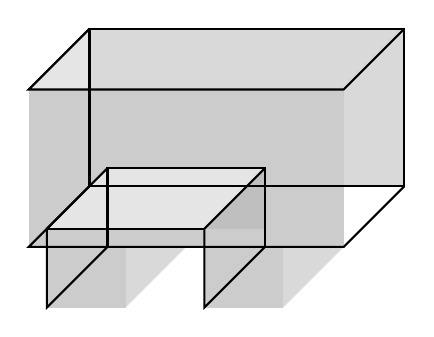
\begin{tikzpicture}[scale=1]

			      % 底部立方体的前侧面
			      \fill[gray!30] (0,0,0) -- (4,0,0) -- (4,2,0) -- (0,2,0) -- cycle; % 前面
			      \fill[gray!20] (0,0,0) -- (0,2,0) -- (0,2,2) -- (0,0,2) -- cycle; % 左面
			      \fill[gray!40] (0,0,2) -- (4,0,2) -- (4,2,2) -- (0,2,2) -- cycle; % 顶面

			      % 凹陷部分左侧立方体
			      \fill[gray!50] (1,0,2) -- (1,1,2) -- (1,1,4) -- (1,0,4) -- cycle; % 左前面
			      \fill[gray!30] (1,0,2) -- (2,0,2) -- (2,0,4) -- (1,0,4) -- cycle; % 左顶面
			      \fill[gray!40] (1,0,4) -- (2,0,4) -- (2,1,4) -- (1,1,4) -- cycle; % 左侧上方面

			      % 凹陷部分右侧立方体
			      \fill[gray!50] (3,0,2) -- (3,1,2) -- (3,1,4) -- (3,0,4) -- cycle; % 右前面
			      \fill[gray!30] (3,0,2) -- (4,0,2) -- (4,0,4) -- (3,0,4) -- cycle; % 右顶面
			      \fill[gray!40] (3,0,4) -- (4,0,4) -- (4,1,4) -- (3,1,4) -- cycle; % 右侧上方面

			      % 凹陷部分底面
			      \fill[gray!20] (1,1,2) -- (3,1,2) -- (3,1,4) -- (1,1,4) -- cycle; % 凹底部面

			      % 边线
			      \draw[thick] (0,0,0) -- (4,0,0) -- (4,2,0) -- (0,2,0) -- cycle; % 底部前边线
			      \draw[thick] (0,0,0) -- (0,0,2) -- (4,0,2) -- (4,0,0);           % 底部顶面边线
			      \draw[thick] (0,2,0) -- (0,2,2) -- (4,2,2) -- (4,2,0);           % 底部后面边线

			      \draw[thick] (1,0,2) -- (1,1,2) -- (3,1,2) -- (3,0,2);           % 凹顶部边线
			      \draw[thick] (1,0,2) -- (1,0,4) -- (1,1,4) -- (1,1,2);           % 凹左侧边线
			      \draw[thick] (3,0,2) -- (3,0,4) -- (3,1,4) -- (3,1,2);           % 凹右侧边线
			      \draw[thick] (1,1,4) -- (3,1,4);                                 % 凹顶横线

		      \end{tikzpicture}
	\end{enumerate}
	\question
	\begin{enumerate}[label=(\arabic*)]
		\item 解不等式: \( \frac{x^2 - x - 6}{x^2 + 2x + 2} < 0 \).
		      \begin{solution}
			      化简得:
			      \begin{math}
				      \frac{x^2 - x - 6}{x^2 + 2x + 2}  = \frac{(x-3)(x+2)}{(x+1)^2 + 1}
			      \end{math}

			      因为分母 \( (x+1)^2 + 1  \)肯定大于0,所以有 \( (x-3)(x+2) < 0 \)

			      因此有 \( -2 < x < 3 \)
		      \end{solution}

		\item 证明: \( \dfrac{2\cos\theta - \sin2\theta}{2\cos\theta + \sin2\theta} = \tan^2\left(\dfrac{90^\circ -
			      \theta}{2}\right) \).
		      \begin{solution}
			      \begin{enumerate}[label=\arabic*. ]
				      \item 首先,根据倍角公式 \( \sin2\theta = 2\sin\theta\cos\theta \) 来化简等式的左边:
				            \begin{align*}
					            \frac{2\cos\theta - \sin2\theta}{2\cos\theta + \sin2\theta}
					             & = \frac{2\cos\theta - 2\sin\theta\cos\theta}{2\cos\theta + 2\sin\theta\cos\theta} \\
					             & = \frac{1-\sin\theta}{1+\sin\theta} \tag{a}
				            \end{align*}
				      \item 然后,结合半角公式 \( \tan\dfrac{\theta}{2} = \dfrac{\sin\theta}{1+\cos\theta} \)
				            来化简等式的右边:
				            \begin{align*}
					            \tan^2\left(\dfrac{90^\circ - \theta}{2}\right)
					             & = \left(\frac{\sin(90^\circ-\theta)}{1+\cos(90^\circ-\theta)}\right)^2 \tag{b}
				            \end{align*}
				      \item 利用差角公式 \( \sin(\alpha-\beta) = \sin\alpha\cos\beta - \cos\alpha\sin\beta \) 及 \(
				            \cos(\alpha - \beta) = \cos\alpha\cos\beta + \sin\alpha\sin\beta \) 进一步化简式(b):
				            \begin{align*}
					            \left(\frac{\sin(90^\circ-\theta)}{1+\cos(90^\circ-\theta)}\right)^2
					             & = \left(\frac{\sin90^\circ\cos\theta -
						            \cos90^\circ\sin\theta}{1+\cos90^\circ\cos\theta + \sin90^\circ\sin\theta}\right)^2
					            \\
					             & = \left(\frac{\cos\theta}{1+\sin\theta}\right)^2 \\
					             & = \frac{\cos^2\theta}{(1+\sin\theta)^2}          \\
					             & = \frac{1-\sin^2\theta}{(1+\sin\theta)^2}        \\
					             & = \frac{1-\sin\theta}{1+\sin\theta} \tag{c}
				            \end{align*}
				      \item 综上,由(a) = (c),原式成立.
			      \end{enumerate}
		      \end{solution}
		\item
		      某中学革命师生自己动手油漆一个直径为$1.2$米的地球仪,如果第平方米面积需要油漆$150$克,问共需油漆多少克?(答案保留整数.)
		      \begin{solution}
			      球体的面积公式为: \( A = 4\pi r^3 \),代入$r=1.2$得:
			      \begin{math}
				      A = 4\times 3.14 \times 1.2^2 = 18.0864
			      \end{math}

			      则共需油漆 \( 18.0864 \times 150 = 2712.96 \approx 2713 \text{g} \)
		      \end{solution}
		\item
		      某农机厂开展\enquote{工业学大庆}运动,在十月份生产拖拉机$1000$台,这样,一月至十月的产量恰好完成全年生产任务.工人同志为了加速农业机械化,计划在年底前再生产$2310$台,求十一月、十二月平均每月增长率.

		      \begin{solution}
			      设每月的平均增长率为$x$,则有 	\( 1000(1+x) + 1000(1+x)^2 = 2310 \).
			      对式子进行化简:
			      \begin{align*}
				      1000(1+x) + 1000(1+x)^2 & = 1000 + 1000x + 1000 + 2000x + 1000x^2 \\
				                              & = 2000 + 3000x + 1000x^2 = 2310         \\
				      1000x^2 +3000x - 310    & = 0                                     \\
				      (10x + 31)(100x - 10)   & = 0                                     \\
				      x                       & = 10\%
			      \end{align*}
		      \end{solution}
	\end{enumerate}
	\question 在半径为$R$的圆内接正六边形内,依次连续各边的中点,得一正六边形,又在这一正六边形内,再依次连结各边的中点,又得一正六边形,这样无限地继续下去,求:
	\begin{enumerate}[label=(\arabic*)]
		\item 前$n$个正六边形的周长之和$S_n$;
		\item 所有这些正六边形的周长之和$S$.
	\end{enumerate}
	\begin{solution}
		\begin{enumerate}[label=\zhnum{*}、]
			\item 半径为$R$的圆的内接正六边形的边长也为$R$,所以第一个正六边形的边长为$6R$.
			\item
			      以第一个正六边形的边的中点连接而成的第二个正六边形的边长,根据三角关系得到边长为\\$\dfrac{\sqrt{3}}{2}R$,则边长为$3\sqrt{3}R$
			\item 则前$n$个正六边形的周长之和为:
			      \begin{align*}
				      S_n & = 6R + 3\sqrt{3}R + \cdots +  (\frac{\sqrt{3}}{2})^{n-1}R \\
				          & = 12\frac{1-(\frac{\sqrt{3}}{2})^n}{2-\sqrt{3}}R          \\
			      \end{align*}
			\item 所有这些正六边形的周长之和:
			      \begin{align*}
				      S & = \lim_{n\to\infty}12\frac{1-(\frac{\sqrt{3}}{2})^n}{2-\sqrt{3}}R \\
				        & = \frac{12}{2-\sqrt{3}}R                                          \\
				        & = 12(2+\sqrt{3})R
			      \end{align*}
		\end{enumerate}
	\end{solution}

	\question 动点$P(x,y)$到两定点$A(-3,0)$和$B(3,0)$的距离的比等于$2$,求动点$P$的轨迹方程,并说明这轨迹是什么图形.
	\begin{solution}
		\begin{enumerate}[label=\arabic*.]
			\item
			      由题意得:
			      \begin{equation*}
				      \sqrt{(x+3)^2 + y^2} = 2\sqrt{(x-3)^2 + y^2}
			      \end{equation*}
			\item
			      方程两边平方得:
			      \begin{equation*}
				      x^2 + 6x + 9 + y^2 = 4x^2 - 24x + 36 + 4y^2
			      \end{equation*}
			\item 进一步整理得$P$的轨迹方程:
			      \begin{equation*}
				      (x-5)^2 + y^2 = 16
			      \end{equation*}
			\item 这个轨迹是圆心在$(5,0)$,直径为$4$的圆.
		\end{enumerate}
	\end{solution}

	\question 某大队在农田基本建设的规划中,要测定被障碍物隔开的两点$A,
		P$之间的距离,他们土法上马,在障碍物的两侧,选取两点$B$和$C$(如图),测得$AB=AC=50$m,$ \angle{BAC}=60^\circ,
		\angle{ACP}=120^\circ, \angle{ACP}=135^\circ$,求$A$和$P$之间的距离.(答案可用最简根式表示).

	\begin{figure}[htbp]
		\centering
		\begin{tikzpicture}[scale=1.5]
			\tkzDefPoint(0,0){A}
			\tkzDefShiftPointCoord[A](30:2){C}
			\tkzDefShiftPointCoord[A](-30:2){B}
			\tkzDefPoint(4,0.3){P}
			\tkzInterLL(A,P)(B,C) \tkzGetPoint{D}
			\tkzDefLine[orthogonal=through C](B,P) \tkzGetPoint{x}
			\tkzInterLL(B,P)(C,x) \tkzGetPoint{E}
			\tkzInterLL(A,P)(C,E) \tkzGetPoint{O}

			\tkzDrawPolygon(A,B,P,C)
			\draw[fill=gray!50] (D) ellipse[x radius=0.3, y radius=0.2];
			\tkzDrawSegments[dashed](A,P B,C)
			\tkzDrawSegment[red, dashed](C,E)
			\tkzDrawPoint(O)

			\tkzLabelAngle[pos=.8](E,C,P){$45^\circ$}
			\tkzMarkAngle[size=.5, mark=s|](E,C,P)
			\tkzMarkRightAngle[red](C,E,P)

			\tkzMarkAngle[size=.5, mark=s|](C,P,E)
			\tkzLabelAngle[pos=.8](C,P,E){$45^\circ$}

			\tkzMarkAngle[size=.6](B,C,E)
			\tkzLabelAngle[pos=.8](B,C,E){$30^\circ$}
			\tkzMarkRightAngle[red](A,C,E)

			\tkzLabelPoint[left](A){$A$}
			\tkzLabelPoint[below](B){$B$}
			\tkzLabelPoint[above](C){$C$}
			\tkzLabelPoint[right](P){$P$}
			\tkzLabelPoint[below](E){$E$}
			\tkzLabelPoint[above right](O){$O$}

			\tkzLabelSegment[above left](A,C){$x$}
			\tkzLabelSegment[below left](A,B){$x$}
			\tkzLabelSegment[below right](B,E){$\frac{x}{2}$}
			\tkzLabelSegment[below right](E,P){$\frac{\sqrt{3}}{2}x$}
		\end{tikzpicture}
	\end{figure}

	\begin{solution}
		\begin{enumerate}[label=\zhnum{*}、, noitemsep]
			\item 为了书写方便,将$AC$的长度记为$x$
			\item 由于 \( AB=AC\)且\( \angle{BAC}=60^\circ \),得 \( \triangle{ABC}是等边三角形 \),并有 \( BC=AB=AC=x \)
			\item 从$C$点作垂线到$BP$并与$BP$,垂足记为$E$,$CE$与$AP$交于$O$点
			\item 由 \( \angle{BAC}=60^\circ, \angle{ACP}=135^\circ, \angle{ABP}=120^\circ \)得$\angle{CPB}=45^\circ$
			\item 则有 \( \angle{ECP} = 45^\circ, \angle{BCE}=30^\circ \)
			\item 由 \( \angle{ACB}=60^\circ, \angle{BCE}=30^\circ \)得 \( \angle{ACO}=90^\circ \)
			\item 在 直角\( \triangle{BCE} \)中,有 \( BE=\frac{BC}{2} = \frac{x}{2}, CE=\frac{\sqrt{3}}{2}BC =
			      \frac{\sqrt{3}}{2}x \)
			\item 在等腰直角三角形 \( \triangle{EPC} \)中,有 \( EP = EC = \frac{\sqrt{3}}{2}x \)
			\item 对于 \( \triangle{ACO} \)和 \( \triangle{PEO} \),因为 \( \angle{ACO} = \angle{PEO} = 90^\circ,
			      \angle{AOC} = \angle{POE} \),所以 \( \triangle{AOC} \sim \triangle{POE} \)

			      根据相似三角形的性质有:
			      \begin{align*}
				      \frac{AC}{EP}                 & = \frac{CO}{OE} = \frac{AO}{OP}                     \\
				      \frac{x}{\frac{\sqrt{3}}{2}x} & = \frac{CO}{OE} = \frac{AO}{OP}= \frac{2}{\sqrt{3}} \\
			      \end{align*}
			\item 因为 \( CE=\frac{\sqrt{3}}{2}x \),则有 \( CO = (2\sqrt{3} - 3)x, OE = \frac{6 - 3\sqrt{3}}{2}x \)
			\item 则有 \( AO = \sqrt{AC^2 + CO^2} = \sqrt{x^2 - (2\sqrt{3} - 3)^2x^2} = \sqrt{12\sqrt{3} - 20}x \)
			\item
			      \begin{align*}
				      OP & = \frac{\sqrt{3}}{2} \cdot AO               \\
				      AP & = AO + OP                                   \\
				         & = (1+\frac{\sqrt{3}}{2})AO                  \\
				         & = \frac{2+\sqrt{3}}{2}\sqrt{12\sqrt{3}-20}x \\
				         & = \sqrt{\sqrt{3} + 1}x                      \\
				         & = 50\sqrt{\sqrt{3} + 1}
			      \end{align*}

		\end{enumerate}
	\end{solution}

	\question 已知双曲线 \( \frac{x^2}{24\tan\alpha} - \frac{y^2}{16\cot\alpha} = 1 (\alpha\text{为锐角})\)和圆 \( (x-m)^2 +
	y^2 = r^2 \)相切于点 \( A(4\sqrt{3},4) \),求 \( \alpha, m, r \)的值.
	\begin{solution}
		\begin{enumerate}[label=\arabic*., noitemsep]
			\item 将点 	\( A(4\sqrt{3}, 4) \)代入双曲线方程得:
			      \begin{equation*}
				      \frac{(4\sqrt{3})^2}{24\tan\alpha} - \frac{4^2}{16\cot\alpha} = 1
			      \end{equation*}

			      进一步化简得:
			      \begin{equation*}
				      \frac{2}{\tan\alpha} - \frac{1}{\cot\alpha} = 1
			      \end{equation*}
			      设 $\tan\alpha=x$,则有:
			      \begin{align*}
				      2\cdot\frac1x - x = 1 \\
				      x^2 +x - 2 = 0        \\
				      (x+2)(x-1) = 0        \\
			      \end{align*}
			      因为$\alpha$是锐角,所以 $x=1$,即 \( \alpha=45^\circ \).
			\item 将点 \( A(4\sqrt{3}, 4) \)代入圆方程得:
			      \begin{equation*}
				      (4\sqrt{3} - m)^2 + 4^2 = r^2 \tag{a}
			      \end{equation*}
			\item 双曲线与圆在 $A$点相切,所以其切线斜率相同.
			      \begin{enumerate}[label=\alph*., noitemsep]
				      \item 求解双曲线在$A$点的切线的斜率

				            对双曲线求偏导:
				            \begin{equation*}
					            \frac{2x}{24\tan\alpha} - \frac{2y}{16\cot\alpha}\cdot\frac{\text{d}y}{\text{d} x} = 0
				            \end{equation*}
				            解得:
				            \begin{equation*}
					            \frac{\text{d}y}{\text{d}x} = \frac{\frac{x}{12\tan\alpha}}{\frac{y}{8\cot\alpha}}
					            = \frac{8\cot\alpha\cdot x}{12\tan\alpha\cdot y} = \frac{2x}{3y}
				            \end{equation*}
				            点 \( A(4\sqrt{3},4) \)的切线斜率为:
				            \begin{equation*}
					            k_1 = \frac{2\cdot4\sqrt{3}}{3\cdot4} =
					            \frac{2\sqrt{3}}{3}
				            \end{equation*}
				      \item 求解圆在$A$点的法线的斜率

				            对圆求偏导:
				            \begin{equation*}
					            2(x-m) + 2y\frac{\text{d}y}{\text{d}x} = 0
				            \end{equation*}

				            点$A(4\sqrt{3},4)$处的切线斜率为:
				            \begin{equation*}
					            k_2 = -\frac{4\sqrt{3} - m}{4}
				            \end{equation*}

				      \item 因为 \( k_1 = k_2 \),所以有
				            \begin{align*}
					            -\frac{4\sqrt{3} - m }{4} = \frac{2\sqrt{3}}{3}
				            \end{align*}
				            解得:
				            \begin{math}
					            m = \frac{20}{\sqrt{3}}
				            \end{math}

			      \end{enumerate}

			\item 将 \( m = \frac{20}{\sqrt{3}} \)代入式(a)得:
			      \begin{math}
				      r = \sqrt{\dfrac{112}{3}}
			      \end{math}

		\end{enumerate}
	\end{solution}

	\question 设数列 $1,2,4, \cdots$前$n$项和是$S_n = a + bn + cn^2 +
		dn^3$,求这数列的通项$a_n$的公式,并确定$a,b,c,d$的值.
	\begin{solution}
		\begin{enumerate}[label=\arabic*.]
			\item $a_n = S_n - S_{n-1}$
			      代入并化简:
			      \begin{align*}
				      a_n & = a + bn + cn^2 + dn^3 - a - b(n-1) - c(n-1)^2 - d(n-1)^3 \\
				          & = b + 2cn -c + dn^3 -d(n^3 -3n^2 + 3n - 1)                \\
				          & = b - c + d + (2c - 3d)n + 3dn^2
			      \end{align*}
			\item 根据题目中的条件有:
			      \begin{align*}
				      a_0 & = 1 = b - c + d \tag{1}                               \\
				      a_1 & = 2 = b - c + d + 2c - 3d + 3d = b + c + d\tag{2}     \\
				      a_2 & = 4 = b - c + d + 4c - 6d + 12d = b + 3c + 7d \tag{3}
			      \end{align*}
			      式(2) - 式(1)得 \[c=\frac12 \tag{4}\]
			      将$c=\frac12$代入式(1)得 \[b+d=\frac32\tag{5}\]
			      综合式(3)、(4)、(5)得
			      \begin{align*}
				      b & = \frac43 \\
				      d & = \frac16
			      \end{align*}
			      另外因为$a_0 = a$,所以$a=1$.
			\item 综上,$a,b,c,d$的值分别为:
			      \begin{align*}
				      a & = 1       \\
				      b & = \frac43 \\
				      c & = \frac12 \\
				      d & = \frac16
			      \end{align*}
			      $a_n$的通项公式为:
			      \begin{equation*}
				      a_n = \frac12n^2 + \frac12n + 1
			      \end{equation*}

		\end{enumerate}

	\end{solution}
	\begin{center}
		\section*{附加题}
	\end{center}
	\question 求函数 $y = e^{-2x}\sin\left(5x+\dfrac{\pi}{4}\right)$的导数.
	\begin{solution}
		\begin{align*}
			\frac{\mathrm{d}y}{\mathrm{d}x} & =  (e^{-2x})'\sin\left(5x + \frac{\pi}{4}\right) + e^{-2x}\sin'\left(5x +
			\frac{\pi}{4}\right)                                                                                        \\
			                                & = -2e^{-2x}\sin\left(5x+\frac{\pi}{4}\right) +
			5e^{-2x}\cos\left(5x+\frac{\pi}{4}\right)                                                                   \\
			                                & = e^{-2x}\left[-2\sin\left(5x + \frac{\pi}{4}\right) + 5\cos\left(5x +
			\frac{\pi}{4}\right)\right]                                                                                 \\
			                                & = e^{-2x}\left[-2\sin5x\cos\frac{\pi}{4} - 2\cos5x\sin\frac{\pi}{4} +
			5\cos(5x)\cos(\frac{\pi}{4}) - 5\sin(5x)\sin(\frac{\pi}{4})\right]                                          \\
			                                & = -\frac{\sqrt{2}}{2}e^{-2x}[7\sin(5x) - 3\cos(5x)]
		\end{align*}
	\end{solution}

	\question 求定积分:$\int_0^1\left(xe^{x^2} + x^2e^2\right)\mathrm{d}x$
	\begin{solution}
		\begin{enumerate}[label=\arabic*.]
			\item 根据和差积分法则有:
			      \begin{equation*}
				      \int_0^1\left(xe^{x^2} + x^2e^2\right)\mathrm{d}x  = \int_0^1(xe^{x^2})\,\mathrm{d}x + \int_0^1(x^2e^2)\,\mathrm{d}x
			      \end{equation*}
			\item 先求解 $\int_0^1(xe^{x^2})\,\mathrm{d}x $,设 $u=x^2$,则有$\mathrm{d}u=2x\mathrm{d}x$,则有
			      \begin{align*}
				      \int_0^1(xe^{x^2})\mathrm{d}x & = \frac12\int_0^1e^u\mathrm{d}u \\
				                                    & = \frac12(e-1)
			      \end{align*}
			\item 再来求解 $\int_0^1(x^2e^2)\,\mathrm{d}x$
			      \begin{align*}
				      \int_0^1(x^2e^2)\,\mathrm{d}x & = e^2\int_0^1x^2\mathrm{d}x \\
				                                    & = \frac{e^2}{3}
			      \end{align*}
			\item 将两部分加起来得到总的积分值:
			      \begin{equation*}
				      \frac12(e-1) + \frac{e^2}{3}
			      \end{equation*}
		\end{enumerate}
	\end{solution}
\end{questions}
